\documentclass{beamer}
\usetheme{Gelugor}

\usepackage[utf8]{inputenc}
\usepackage{amsmath}
\usepackage{mathtools}
\usepackage[T1]{fontenc}
\usepackage{lipsum}
%% Use any fonts you like.
\usepackage{helvet}
\usepackage{caption}
\usepackage{graphicx}
\usepackage{animate}
%comment
\newcommand{\comment}[1]{}

%% Use tikz extention
\usepackage{tikz}
\usetikzlibrary{arrows,shapes,trees}
\definecolor{gold}{rgb}{0.85,0.65,0}

\title{Melacak Sampah Plastik dengan Analisis Laut Lagrangian Menggunakan OceanParcels}
%\subtitle{Click Here to Add Subtitle}
\author{Muh. Nur Hidayat}
\date{\today}
\institute{----\\ Pembimbing 1: Prof. Dr. Ir. Syamsul Rizal \\Pembimbing 2: Prof. Dr. Marwan Ramli, M.Si.}

\begin{document}

\begin{frame}[plain,t]
\titlepage

\end{frame}


\section{Daftar Isi}
\begin{frame}
\frametitle{Daftar Isi}
\framesubtitle{Table of Contents}
\begin{itemize}
\item Pendahuluan
	\begin{itemize}
	\item Latar Belakang dan Rumusan Masalah
	\item Tujuan Penelitian
	\item Urgensi dan Kebaruan Penelitian
	\item Manfaat Penelitian
	\end{itemize}
\item Tinjauan Pustaka
	\begin{itemize}
	\item Persamaan Gerak Fluida
	\item Persamaan Navier-Stokes 3 Dimensi
	\item Analisis Laut Lagrangian
	\item OceanParcels
	\item Arakawa C-grid
	\end{itemize}
\item Metodologi Penelitian
	\begin{itemize}
	\item Domain Penelitian
	\item Data Penelitian
	\item Prosedur Penelitian
	\end{itemize}
\end{itemize}
\end{frame}

\section{Pendahuluan}
\subsection{Latar Belakang dan Rumusan Masalah}
\begin{frame}[allowframebreaks]
\frametitle{Latar Belakang dan Rumusan Masalah}
	\lipsum[75]
	\begin{figure}[H]
		\centering
		\includegraphics[width=10cm]{Where-does-plastic-accumulate.png}
		\caption{Distribusi sampah plastik di laut (Ritchie \& Roser, 2018)}
		\label{fig:plasticdata}
	\end{figure}
	\lipsum[66]
\end{frame}

\subsection{Tujuan Penelitian}
\begin{frame}
\frametitle{Tujuan Penelitian}
	\begin{itemize}
		\item Menginvestigasi sebaran sampah mikroplastik yang berasal dari perairan Aceh
		\item Mengkaji model numerik analisis laut lagrangian
		\item Mencari hubungan antara kecepatan zonal dan meridional, dan gaya angin terhadap lintasan mikroplastik.
	\end{itemize}
\end{frame}

\subsection{Urgensi dan Kebaruan Penelitian}
\begin{frame}
	\frametitle{Urgensi dan Kebaruan Penelitian}
	\begin{itemize}
		\item Untuk mengetahui cara kerja dari alat yang digunakan + analisis matematis terkait penelitian lanjutan
		\item Aplikasi OceanParcels dalam domain penelitian belum pernah diteliti sebelumnya
		\item Untuk mengetahui hubungan-hubungan gaya yang bekerja di dalamnya.
	\end{itemize}
\end{frame}

\subsection{Manfaat Penelitian}
\begin{frame}
	\frametitle{Manfaat Penelitian}
	\begin{itemize}
		\item Diharapkan mampu menjawab salah satu tantangan terkait sampah plastik dan cara penanggulangannya dengan mengetahui sebaran sampah plastik yang berasal dari wilayah sasaran penelitian.
		\item Penjabaran model numerik yang dilakukan akan menambah pengetahuan matematis serta dapat memperoleh gambaran tentang cara kerja model, dan potensi penelitian lanjutan.
	\end{itemize}
\end{frame}

\section{Tinjauan Pustaka}
\subsection{Persamaan Gerak Fluida}
\begin{frame}
	\frametitle{Persamaan Gerak Fluida}
	\begin{figure}[H]
		\centering
		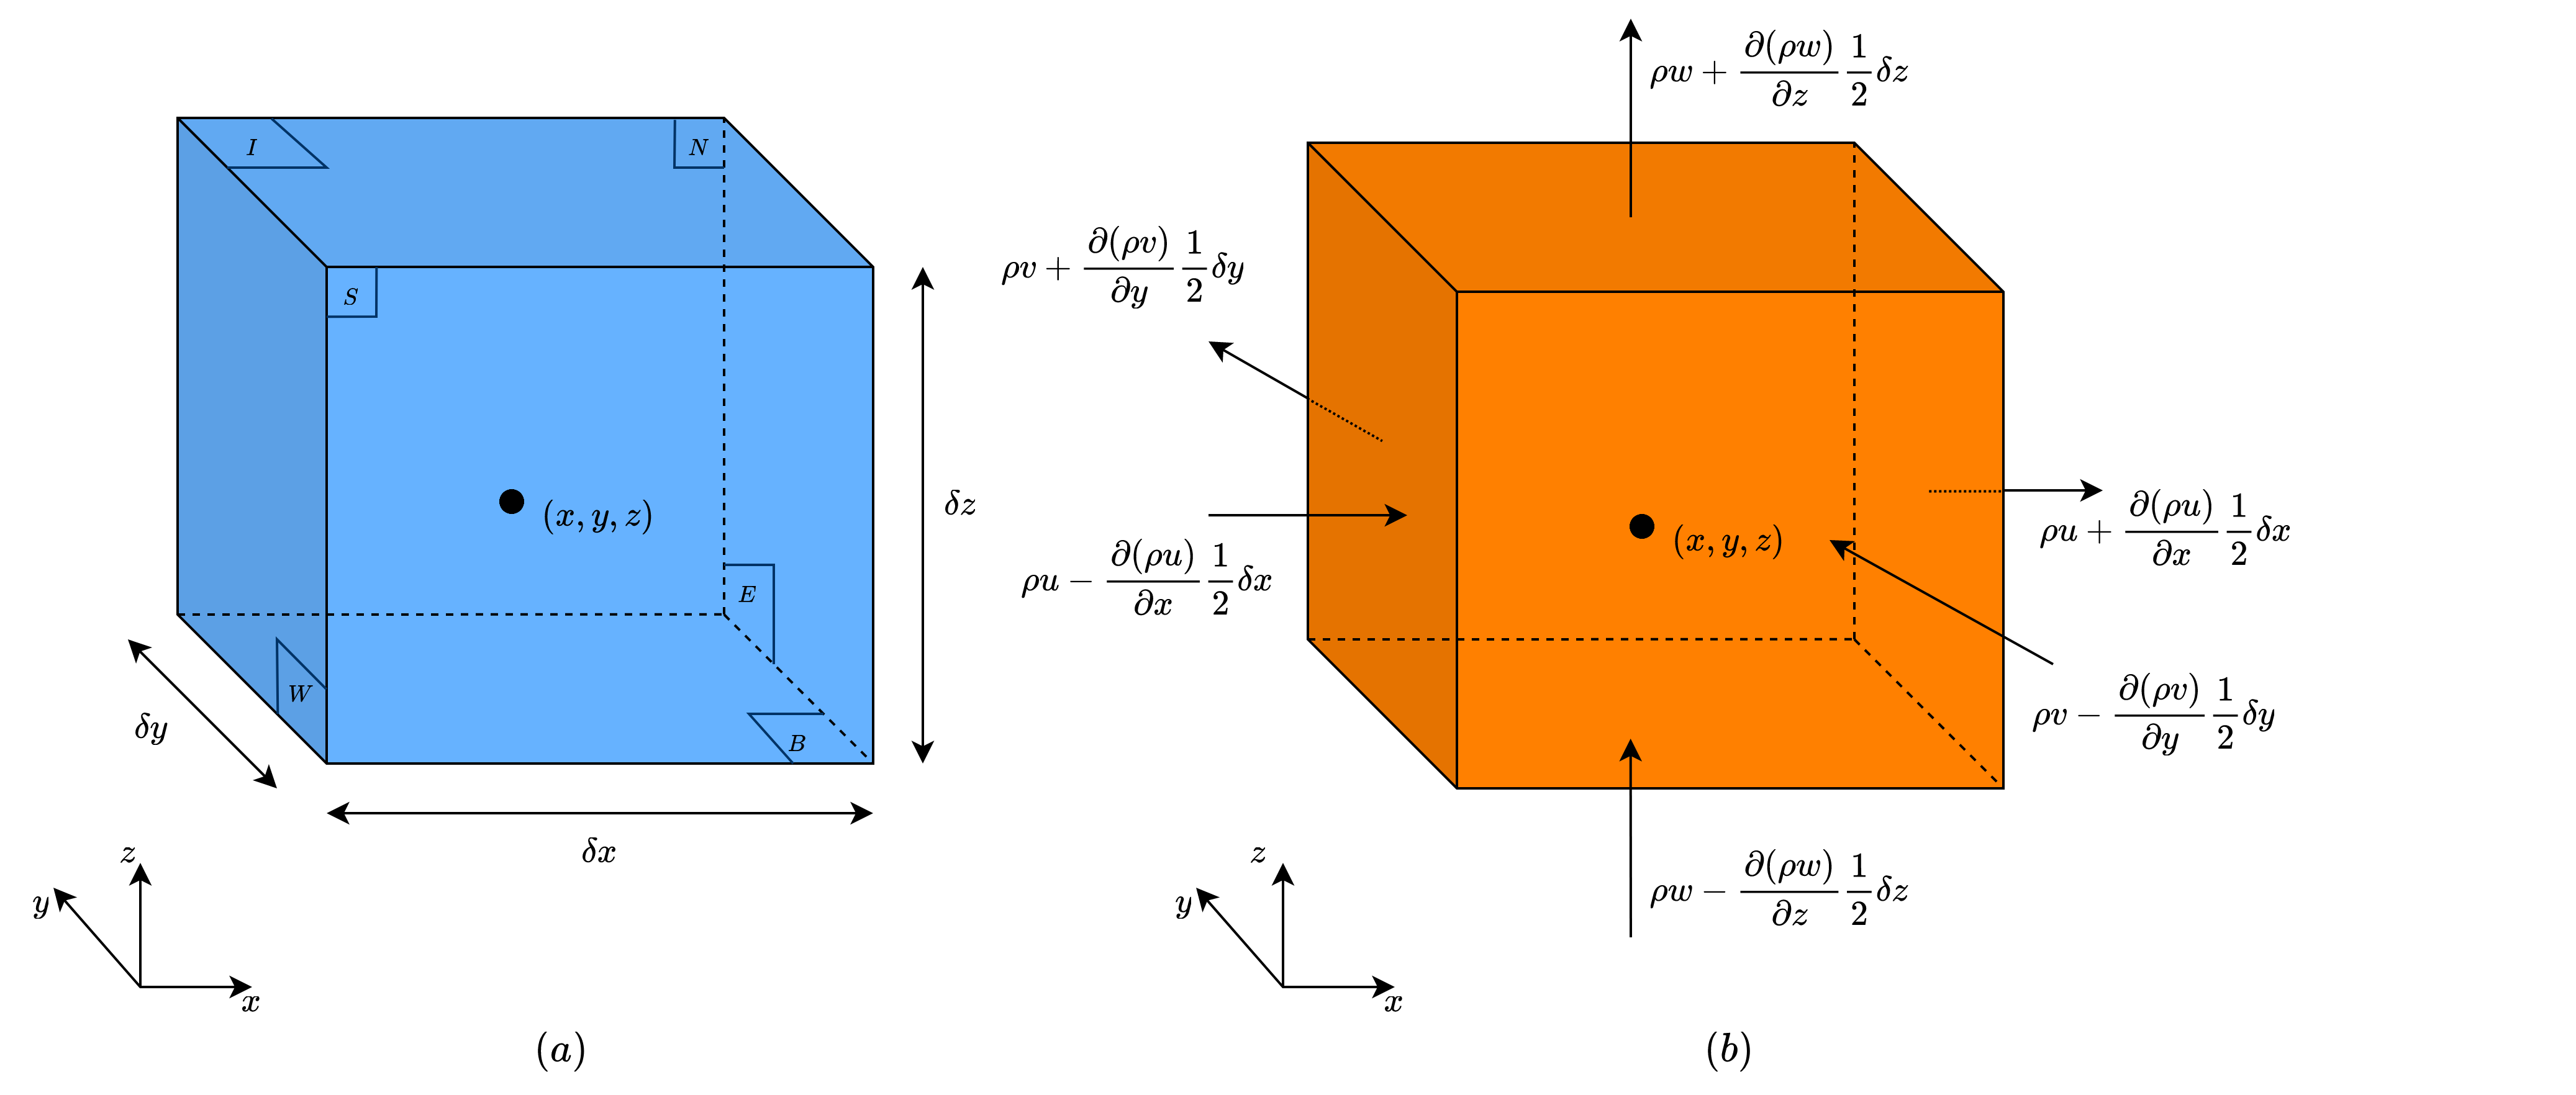
\includegraphics[width=10cm]{cube.png}
		\caption{(a) Ilustrasi partikel sebagai sifat fisis fluida. (b) Aliran massa jenis masuk
			dan keluar (Versteeg \& Malalasekera, 2007)}
		\label{fig:cube}
	\end{figure}
\end{frame}

\subsection{Persamaan Navier-Stokes 3 Dimensi}
\begin{frame}[allowframebreaks]
	\frametitle{Persamaan Navier-Stokes 3 Dimensi}
	Model OGCM $\rightarrow$ persamaan Navier-Stokes: 
	\begin{itemize}
		\item Persamaan momentum.
		\item Persamaan kontinuitas.
		\item Persamaan konservasi densitas.
	\end{itemize}
	Model Navier-Stokes dengan pendekatan nonhidrostatik, 
	\begin{equation}
		P = p+q.
	\end{equation}
	Tekanan p dihitung secara diagnostik dari densitas  dan percepatan gravitasi g seperti pada persamaan berikut 
	\begin{equation}
		\frac{\partial p}{\partial z} = -(\rho - \rho_0)g.
	\end{equation}
	Sedangkan tekanan q dihitung secara prognostik dalam persamaan momentum (implisit). \\ $\;$ \\
	Persamaan momentum,
	\begin{equation}
		\begin{aligned}
			\frac{\partial u}{\partial t} + \text{adv}(u)-fv &= \frac{-1}{\rho_0}\frac{\partial(p+q)}{\partial x}+\text{diff}(u) \\
			\frac{\partial v}{\partial t} + \text{adv}(v)+fu &= \frac{-1}{\rho_0}\frac{\partial(p+q)}{\partial y}+\text{diff}(v) \\
			\frac{\partial w}{\partial t} +\text{adv}(w) &= \frac{-1}{\rho_0}\frac{\partial(q)}{\partial y}+\text{diff}(w).
		\end{aligned}	
	\end{equation}
	dengan persamaan adveksi \\ $\text{adv}(\psi)=u\frac{\partial \psi}{\partial x}+v\frac{\partial \psi}{\partial y}+w\frac{\partial \psi}{\partial z}$ \\
	dan persamaan difusi $\text{diff}(\psi)=\frac{\partial}{\partial x}(A_{H} \frac{\partial \psi}{\partial x})+\frac{\partial}{\partial y}(A_{H} \frac{\partial \psi}{\partial y})+\frac{\partial}{\partial z}(A_{Z} \frac{\partial \psi}{\partial z})$
	\newpage 
	Persamaan kontinuitas,
	\begin{equation}
		\frac{\partial u}{\partial t} + \frac{\partial v}{\partial t} + \frac{\partial w}{\partial t} = 0.
	\end{equation}
	Tekanan dinamis pada lapisan permukaan berdasarkan persamaan kontinuitas,
	\begin{equation}
		\frac{\partial q_s}{\partial t} = \rho_0 g_i \times \left( \frac{(\partial \left(H \langle u \rangle \right)} {\partial x} + \frac{(\partial \left(H \langle v \rangle \right)} {\partial y}\right)
	\end{equation}
	Persamaan konservasi densitas,
		\begin{equation}
		\frac{\partial \rho}{\partial t} + \text{adv}(\rho) = \text{diff}(\rho)
	\end{equation}
\end{frame}
	
\subsection{Analisis Laut Lagrangian}
\begin{frame}[allowframebreaks]
	\frametitle{Analisis Laut Lagrangian}
		$\;$ \\
	Konsep yang digunakan untuk mensimulasikan
	pergerakan air di lautan,
	\begin{itemize}
		\item Pendekatan Lagrangian. \\ \vspace{.5pt}
		\tiny Pergerakan partikel dinyatakan dan diobservasi sebagai fungsi waktu dan dianggap bahwa kerangka acuan bergerak bersama-sama dengan partikel fluida, cth: \\ \vspace{-5.5pt} $s(x_0,y_0,z_0,t), V(x_0,y_0,z_0,t), \;\text{dan}\; a(x_0,y_0,z_0,t)$. \normalsize
		\item Pendekatan Eulerian. \\
		\tiny Pergerakan tiap partikel dinyatakan dan diobservasi sebagai fungsi ruang dan waktu dengan kerangka acuan tetap. cth:
		$V = V(x,y,z,t)$
	\end{itemize}
	Tujuan teknis dari analisis laut Lagrangian adalah untuk memperkirakan lintasan partikel virtual fluida dengan memanfaatkan informasi Eulerian fluida, yaitu medan kecepatan (van Sebille et al., 2018). \newpage
	Misal vektor posisi X(t) bergantung terhadap waktu t. \\
	Jika bentuk $n$ partikel diskrit ($n \in \mathbb{N}$), vektor posisi dinotasikan sebagai $X^n(t)$, dan \\
	Jika n kontinu, vektor posisi dinotasikan sebagai $x=X(a,t)$ dimana $a$ adalah koordinat materi, posisi partikel dengan referensi waktu $t=t_0$. \\
	\vspace{5.5pt}
	\par Selanjutnya parsel fluida (molekul skala mikroskopik) dalam bentuk kontinu diformulasikan dengan menghitung turunan lintasan partikel terhadap waktu (a konstan), 
	\begin{equation}\label{eq:basic_traj}
		v(x,t) = \left(\frac{\partial X(a,t)}{\partial t}\right)_a
	\end{equation}
	$\;$ \\
	$\;$ \\
	$\;$ \\
	$\;$ \\
	Untuk memperoleh deskripsi kinematik yang lebih lengkap, misalkan fungsi sembarang $\psi$ yang dihitung disepanjang lintasan, $\psi(X(a,t),t)$. Dengan aturan rantai diperoleh,
	\begin{equation*}
		\begin{aligned}
			\frac{\partial \psi(X(a,t),t)}{\partial t}&=\frac{\partial \psi(X(a,t),t)}{\partial t} + \left(\frac{dX(a,t)}{dt}\right)\frac{\partial \psi(X(a,t),t)}{\partial X(a,t)}  \\
			&= \left[\frac{\partial}{\partial t} + v(X(a,t),t)\frac{\partial}{\partial X(a,t)}\right]\psi(X(a,t),t),
		\end{aligned}
	\end{equation*}
	atau secara umum diperoleh,
	\begin{equation}
		\frac{\partial \psi(X(a,t),t)}{\partial t}=\left[\frac{\partial}{\partial t}+v(X(a,t),t).\nabla\right]\psi(X(a,t),t).
	\end{equation}
	\newpage
	$\;$ \\
	$\;$ \\ 
	Metode integrasi Lagrangian, 
	\begin{itemize}
		\item Secara online. \\ \vspace{.5pt}
		\tiny Lintasan dihitung disetiap langkah waktu sehingga model Eulerian diperbaharui secara terus-menerus (cth software: \href{mpas-dev.github.io}{LIGHT in MPAS-O}, \href{nemo-ocean.eu/About-NEMO/Reference-manuals}{NEMO online floats and icebergs}, \href{mitgcm.org}{MITgcm}, \href{hycom.org}{HYCOM Float Package}, dan \href{myroms.org/wiki/floats.in}{ROMS online floats}) \\ \vspace{-5.5pt} $\;$ \normalsize
		\item Secara offline. \\
		\tiny Perhitungan model offline menawarkan kemampuan untuk menghitung lintasan dalam mode maju (dari titik awal dan maju dalam waktu) atau dalam mode mundur (dari titik akhir dan mundur dalam waktu) (cth software: \href{https://www.univ-brest.fr/lpo/ariane}{Ariane}, \href{tracmass.org}{TRACMASS}, \href{https://github.com/jinbow/Octopus}{Octopus}, \href{https://bitbucket.org/f_nencio/spasso/overview}{LAMTA}, \href{https://github.com/beatrixparis/connectivity-modeling-system}{CMS}, dan \href{oceanparcels.org}{Parcels})
	\end{itemize}
	\newpage
	Proses transportasi dilautan yang mempengaruhi pergerakan dari partikel plastik,
	\begin{itemize}
		\item Stokes drift. \\ \vspace{.5pt}
		\tiny Stokes drift $\overline{u_s}$, diformulasikan sebagai 
		\begin{equation}
			\overline{u_s}=\overline{u_L}-\overline{u_E},
		\end{equation}
		dengan $\overline{u_E},\overline{u_L}$ menyatakan rata-rata kecepatan Eulerian dan Lagrangian, dan
		\begin{equation*}
			\begin{cases}
				\overline{u_E} &= \overline{\frac{\partial x}{\partial t}} = \overline{u(x,t)}, \\
				\overline{u_L} &= \overline{\frac{\partial X(a,t)}{\partial t}} = \overline{u(X(a,t),t)}.
			\end{cases}	
		\end{equation*} 
		Dikarenakan gaya stokes drift, partikel plastik yang terapung dilautan akan memiliki kecepatan dalam arah yang sama dengan perambatan gelombang. Gelombang yang dimaksud adalah gelombang gravitasi permukaan yang muncul dari antarmuka atmosfer dan laut (Brach et al., 2018).
		\\ \vspace{-5.5pt} $\;$ \normalsize
		\item Angin. \\
		\tiny Angin memainkan peran penting dalam mendorong arus permukaan dan juga dalam proses interaksi udara-laut. Sampah mikroplastik dapat ditransportasikan secara langsung oleh gaya angin dan mempengaruhi setiap benda yang berada diatas permukaan air (van Sebille et al., 2020). Sebagian besar proses interaksi udara-laut ditentukan dengan menggunakan tekanan angin (\textit{wind stress}), suatu ukuran transfer momentum yang disebabkan oleh gerakan relatif antara laut dan atmosfer (Chacko et al., 2022). Tekanan angin berdasarkan aerodinamis massal (\textit{bulk-aerodynamic}) dirumuskan sebagai,
		\begin{equation}
			\tau = \rho_a C_d U_w^2
		\end{equation}
		dengan $\rho_a$ adalah densitas udara $(1.225 kg/m^3)$, $C_d$ koefisien seret (\textit{dimensionless}) $(\approx 1.3 \times 10^-3)$ dan $U_w$ kecepatan angin.
	\end{itemize}
\end{frame}

\subsection{OceanParcels}
\begin{frame}[allowframebreaks]
	\frametitle{OceanParcels}	
	\begin{figure}[H]
		\centering
		\includegraphics[width=2cm]{oceanparcel}\;\;
		\animategraphics[width=4cm]{12}{homepageshort-}{0}{19}
	\end{figure}
	\tiny Ocean\textbf{Parcels} (\textbf{P}robably \textbf{A} \textbf{R}eally \textbf{C}omputationally \textbf{E}fficient \textbf{L}agrangian \textbf{S}imulator) adalah kumpulan \textit{class} dan \textit{method} dalam Python untuk membuat simulasi pelacakan partikel yang dapat disesuaikan menggunakan data output dari model sirkulasi laut
	(OGCMs). Parcels dapat digunakan untuk melacak partikel-partikel yang aktif dan pasif seperti air, plankton,plastik, dan ikan. Dalam hal ini, partikel dalam Parcels merepresentasikan berbagai
	benda yang mengapung dan tenggelam di lautan (https://oceanparcels.org/, Lange and
	van Sebille (2017)). 
	\newpage
	\normalsize
	$\;$ \\
	Beberapa projek yang menggunakan Ocean\text{Parcel}: 
	\begin{itemize}
		\item Simulasi plankton yang tenggelam di lautan (plankton-drift.org), (cth: Nooteboom et al., 2019,\& 2020) 
		\item Transportasi mikroba di lautan (Adrift project), (cth: McInnes et al., 2019), 
		\item TOPIOS project untuk membuat peta 3D dari polusi plastik di lautan, (cth: Onink et al., 2019, Lacerda et al., 2019, Iskandar et al., 2021)
	\end{itemize}
	\newpage
	$\;$ \\
	Apabila terdapat $n$ buah partikel yang berlokasi di titik $x=X^{(n)}(t)$, posisi dari partikel dapat diperbaharui dengan mengintegralkan persamaan \ref{eq:basic_traj} dan mengambil langkah waktu kecepatan sehingga
	\begin{equation}\label{eq:traj}
		X(t+\Delta t) = X(t)+\int_{t}^{t+\Delta t}v(x(\tau),\tau)d\tau + \Delta X_b(t),
	\end{equation}
	dengan $\Delta X_b(t)$ adalah tambahan suku di ruas kanan yang merepresentasikan perilaku partikel, seperti contoh daya apung (\textit{buoyancy})(van Sebille et al., 2018). Solusi dari persamaan ini kemudian diaproksimasi dalam Parcels dengan langkah waktu numerik.
	\newpage
	$\;$ \\
	$\;$ \\
	\begin{figure}[H]
		\centering
		\includegraphics[width=7cm]{parcels_flowchart}
		\caption{Flowchart Parcels. Kode disusun dalam tingkat abstraksi tinggi, meminta
			dari pengguna informasi input yang sangat diperlukan (Lange \& van Sebille, 2017)}
		\label{fig:parcelsflowchart}
	\end{figure}
	\newpage
	$\;$ \\
	\textbf{\large Time Stepping} \\
	Persamaan \ref{eq:basic_traj} dan kondisi awal dapat ditulis ulang sebagai 
	\begin{equation}\label{eq:newbasic_traj}
		\dot y(t) = f(t,y(t)), \quad y(t_0)=y_0
	\end{equation}
	dengan posisi partikel pada waktu $t_n$ diberikan  oleh $y(t_n)=(x_n,y_n,z_n)$. Fungsi $f$ adalah kecepatan ($v$) dari partikel yang berbentuk suatu vektor (setiap elemen dalam $f$ adalah kecepatan dalam 1-D). Akibatnya persamaan \ref{eq:traj} (tanpa suku tambahan) menjadi
	\begin{equation}
		y(y_0,t+\Delta t) = y(y_0,t)+\int_{t}^{t+\Delta t}v(y,\tau)d\tau.
	\end{equation}
	$\;$ \\
	$\;$ \\
	$\;$ \\
	Solusi numerik,
	\begin{enumerate}
		\item Metode eksplisit Euler
		\begin{equation}
			y_{n+1}=y_n+hf(t_n,y_n).
		\end{equation}
		\item Metode Runge-Kutta Orde 4 (RK4)
		\[
		\renewcommand\arraystretch{1.2}
		\begin{array}
			{c|cccc}
			0\\
			\frac{1}{2} & \frac{1}{2}\\
			\frac{1}{2} &0 &\frac{1}{2} \\
			1& 0& 0& 1\\
			\hline
			& \frac{1}{6} &\frac{1}{3} &\frac{1}{3} &\frac{1}{6} 
		\end{array}
		\]
		$\;$ \\
		$\;$ \\
		\item Metode Runge-Kutta-Fehlberg (RKF45)
		\[
		\renewcommand\arraystretch{1.2}
		\begin{array}
			{c|cccccc}
			0\\
			\frac{1}{4} & \frac{1}{4}\\
			\frac{3}{8} &\frac{3}{32} &\frac{9}{32} \\
			\frac{12}{13} &\frac{1932}{2197} & -\frac{7200}{2197} & \frac{7296}{2197}\\
			1 &\frac{439}{216} & -8 & \frac{3680}{513} & -\frac{845}{4104}\\
			\frac{1}{2} &-\frac{8}{27} & 2 & -\frac{3544}{2565} & \frac{1859}{4104} & -\frac{11}{40}\\
			\hline
			& \frac{16}{135} &0 &\frac{6656}{12825} &\frac{28561}{56430} & -\frac{9}{50} & \frac{2}{55} \\
			& \frac{25}{216} &0 &\frac{1408}{2565} &\frac{2197}{4104} & -\frac{1}{5} & 0
		\end{array}
		\]
	\end{enumerate}
	$\;$ \\
	$\;$ \\
	Selisih antara orde ke 5 (RK5) dan orde ke 4 (RK4), dihitung dengan cara
	\begin{equation*}
		\kappa = || y_{n+1}^{5th}-y_{n+1}^{4th} ||.
	\end{equation*}
	Persamaan ini digunakan untuk menghitung $\textit{local error}$ di titik $n+1$.
	\newpage
	\textbf{\large Kondisi Batas} \\
	\begin{itemize}
		\item 2-D, kondisi batas antara darat dan laut serta sisi tepi dari domain simulasi yang digunakan.
		\item 3-D, terdapat kedalaman lautan yang mempengaruhi sehingga kondisi batas yang berhubungan adalah antara laut dan dasar laut, atau laut dan permukaan laut.
	\end{itemize}
	Dalam penelitian ini, kondisi batas yang digunakan adalah antara darat dan laut serta sisi tepi dari domain simulasi dan hanya membatasi pada kasus 2-D
\end{frame}

\subsection{Arakawa C-grid}
\begin{frame}[allowframebreaks]
	\frametitle{Arakawa C-grid}	
	\;
	Data OGCM $\xRightarrow{\text{disimpan}}$ \textit{Fields} dalam Parcels yang memuat data 4-Dimensi (longitude, latitude, waktu,  kedalaman) $\xRightarrow{\text{membutuhkan}}$ skema interpolasi dan diskritisasi untuk mendapatkan nilai field
	lokasi partikel.
	\begin{figure}[H]
	\centering
	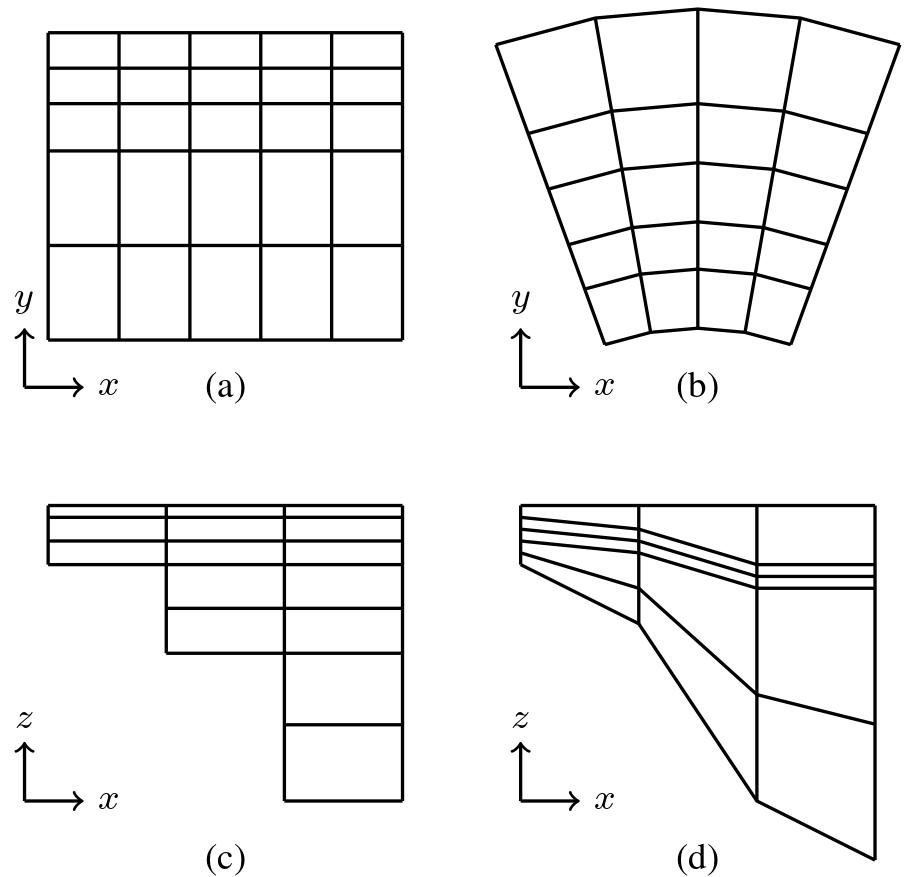
\includegraphics[width=5cm]{grid.jpg}
	\caption{Diskritisasi grid dalam Parcels. Di bidang horizontal: (a) grid persegi, (b) grid lengkung, di bidang vertikal: (c) grid level z, (d) grid level s (Delandmeter \& van Sebille, 2019)}
	\label{fig:grid}
	\end{figure}
	$\;$ \\
	\begin{figure}[H]
		\centering
		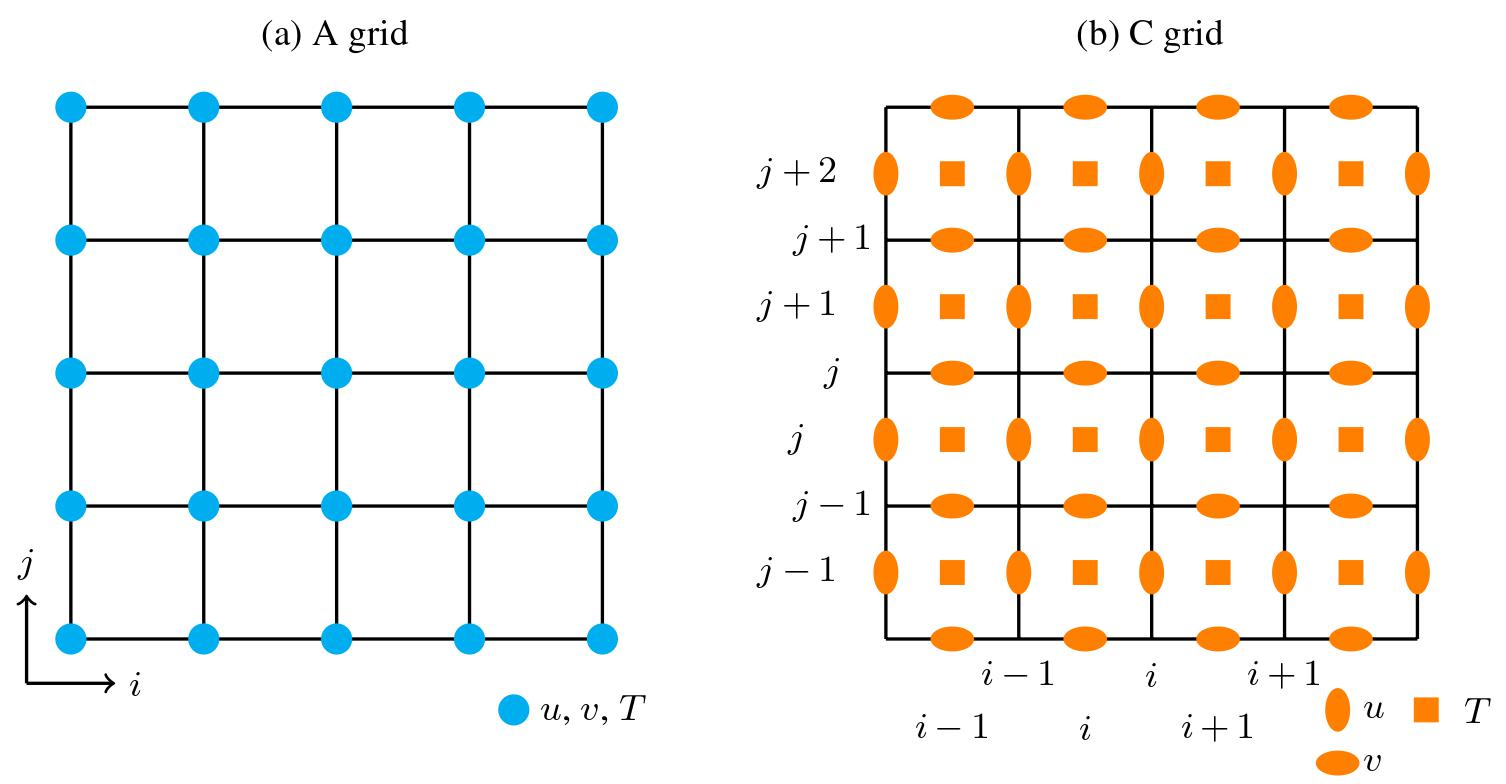
\includegraphics[width=7cm]{arakawa.jpg}
		\caption{Grid Arakawa: (a) Grid A dan (b) Grid C (Delandmeter \& van Sebille, 2019)}
			\label{fig:arakawa}
%			\medspace
			\tiny
			Grid A adalah satu-satunya \textit{unstaggered grid} dalam grid Arakawa dimana variabel-variabelnya (\textit{zonal velocity (u), meridional velocity (v), tracers (T)}) hanya terdapat pada titik sudut grid, berbeda dengan grid C yang berada di sisi dan tengah grid. $i$ dan $j$ adalah indeks yang merepresentasikan variabel kolom dan baris dimana variabel disimpan.
	\end{figure}
	\newpage
	\textbf{\large Bidang 2-D} \\
	\begin{figure}[H]
		\centering
		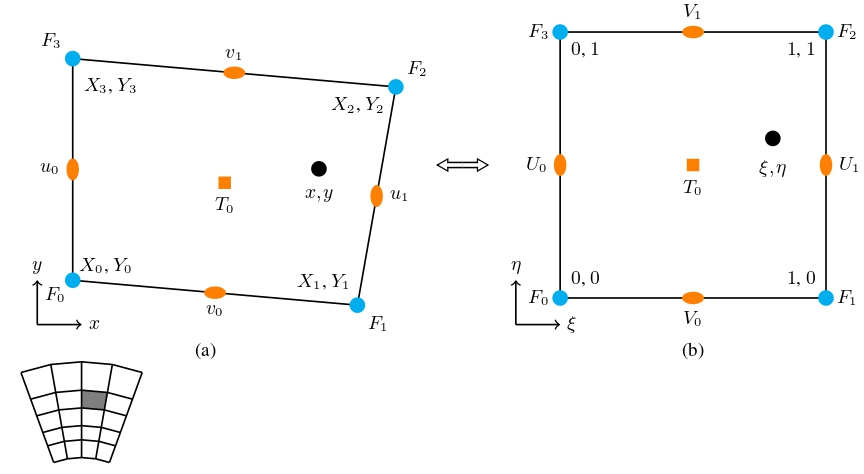
\includegraphics[width=7cm]{mesh_arakawa.jpg}
		\caption{Posisi variabel pada grid A (titik biru), dan grid C (titik jingga) dengan (a) koordinat fisik dalam sel jala (\textit{mesh cell}), (b) koordinat relatif dalam sel satuan (\textit{unit cell}) (Delandmeter \& van Sebille, 2019)}
		\label{fig:mesh}
	\end{figure}
	$\;$ \\
	Definisikan fungsi $f$ sebagai suatu bidang yang diinterpolasi dalam sel $(i,j)$ dengan polinomial Lagrange $\phi_n^{2-D}$ dan 4 titik sentral $F_n, n=0...3$ yang mengelilingi sel, sehingga
	\begin{equation}
		f(x,y)=\sum_{n=0}^{3}\phi_n^{2-D}(\xi,\eta)F_n, 
	\end{equation}
	dengan $\psi, \eta$ memenuhi  
	\begin{equation}\label{eq:xy_2d}
		\begin{cases}
			x &= \sum_n \phi_n^{2-D}(\xi,\eta)X_n \\
			y &= \sum_n \phi_n^{2-D}(\xi,\eta)Y_n.
		\end{cases}	
	\end{equation}
	Polinomial Lagrange 2-D $\phi_n^{2-D}$ untuk $n=0,1,2,3$ menjadi
	\begin{equation*}
		\begin{aligned}
			\phi_0^{2-D} &= (1-\xi)(1-\eta), \quad 	\phi_1^{2-D} &= \xi(1-\eta) \\
			\phi_2^{2-D} &= \xi\eta, \quad 	\quad \quad \quad \quad \quad \phi_3^{2-D} &= (1-\xi)\eta.
		\end{aligned}
	\end{equation*}
	Kecepatan relatif $\xi,\text{dan}\;\eta$ untuk grid A (grid persegi)
		\begin{equation*}
		\begin{aligned}
			\therefore \xi &= \frac{x-X_0}{X_1-X_0}. \\
			\therefore \eta &= \frac{y-Y_0}{Y_3-Y_0}. 
		\end{aligned}
	\end{equation*}
	Komponen kecepatan dari Gambar \ref{fig:arakawa}b dapat ditulis menjadi $(u_0=u_{j+1,i}, u_1=u_{j+1,i+1}, v_0=v_{j,i+1}, v_1=v_{j+1,i+1})$ dan digambarkan sedemikian sebagai Gambar \ref{fig:mesh}a. Kemudian kecepatan pada posisi $(x,y)$ didekati dengan interpolasi linear fluks $(U_0,U_1,V_0,V_1)$ pada sisi-sisi sel (Gambar \ref{fig:mesh}b) sehingga
	\begin{equation}\label{eq:linearflux}
		\begin{cases}
			U_0	= L_{03} u_0, \\
			U_1	= L_{12} u_1, \\
			V_0	= L_{01} v_0, \\
			V_1	= L_{23} v_1, 
		\end{cases}
	\end{equation}
	dengan $L_{03},L_{12},L_{01},\text{dan}\;L_{23}$ adalah panjang sisi sel. Selanjutnya dengan menggunakan persamaan \ref{eq:xy_2d}, misalkan matriks Jacobian 2-D yang mentransformasikan sel fisik menjadi sel satuan pada Gambar \ref{fig:mesh} yang didefinisikan sebagai
	\begin{equation}\label{eq:jacob_2d}
		\begin{aligned}
		\textbf{J}^{2-D}(\xi,\eta)&= \left(\sum_n\frac{\partial \phi_n^{2-D}}{\partial \xi}X_n\right)\left(\sum_n\frac{\partial \phi_n^{2-D}}{\partial \eta}Y_n\right)- \\
		& \left(\sum_n\frac{\partial \phi_n^{2-D}}{\partial \eta}X_n\right) \left(\sum_n\frac{\partial y}{\partial \phi_n^{2-D}}Y_n \right).
		\end{aligned}
	\end{equation}
	
	Determinan dari matriks Jacobian pada persamaan \ref{eq:jacob_2d} selanjutnya dinotasikan $J^{2-D}(\xi,\eta)=\text{det}(\textbf{J}^{2-D})$ dan didefinisikan sebagai rasio antara permukaan dasar dalam sel fisik dan permukaan yang bersesuaian dalam sel satuan. Kecepatan relatif dalam sel satuan didefinisikan sebagai
	\begin{equation}
		\begin{cases}
			\frac{\partial \xi}{\partial t} &= \frac{(1-\xi)U_0+\xi U_1}{J^{2-D}(\xi,\eta)}, \\
			\frac{\partial \eta}{\partial t} &= \frac{(1-\eta)V_0+\eta V_1}{J^{2-D}(\xi,\eta)}.
		\end{cases}	
	\end{equation}
	Dengan mentransformasikan kecepatan relatif kedalam sistem koordinat fisik diperoleh,
	\begin{equation*}
		\begin{aligned}
			u &= \frac{\partial x}{\partial \xi}\frac{\partial \xi}{\partial t}+\frac{\partial x}{\partial \eta}\frac{\partial \eta}{\partial t}, \\
			v &= \frac{\partial y}{\partial \xi}\frac{\partial \xi}{\partial t}+\frac{\partial y}{\partial \eta}\frac{\partial \eta}{\partial t}.
		\end{aligned}	
	\end{equation*}
	\newpage
	\textbf{\large Ruang 3-D} \\
	\begin{figure}[H]
		\centering
		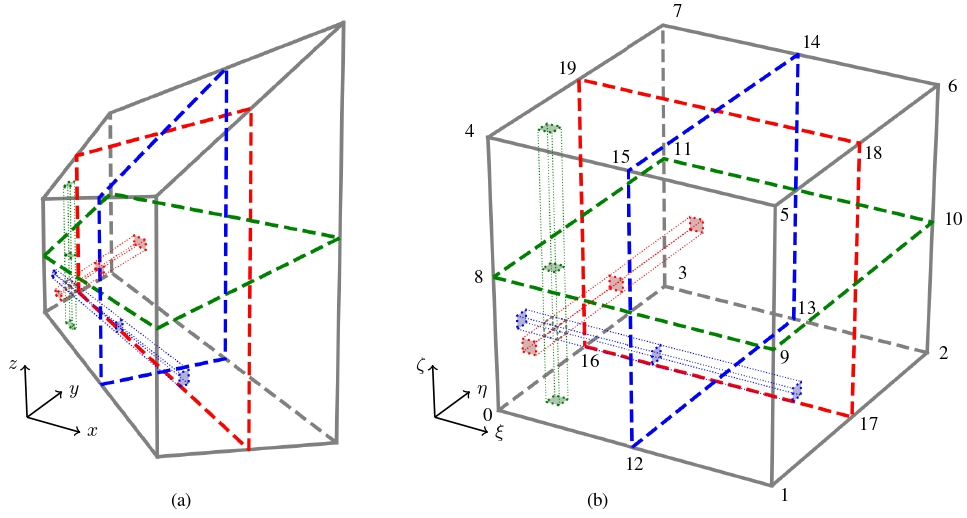
\includegraphics[width=7cm]{mesh_arakawa3d.jpg}
		\caption{Fluks yang digunakan untuk interpolasi 3-D pada grid C Arakawa: (a) sel fisik, (b) sel satuan (Delandmeter \& van Sebille, 2019).}
		\label{fig:mesh3d}
	\end{figure}
	
\end{frame}

\section{Metodologi Penelitian}
\subsection{Domain Penelitian}
\begin{frame}
	\frametitle{Domain Penelitian}
	\begin{figure}[H]
		\centering
		\includegraphics[width=9cm]{area_of_interest}
		\caption{Domain Penelitian}
		\label{fig:domain}
	\end{figure}
\end{frame}

\subsection{Data Penelitian}
\begin{frame}
	\frametitle{Data Penelitian}
	\begin{figure}[H]
		\centering
		
\includegraphics[width=.24\textwidth]{logo_hycom.png} \;\;
		
\includegraphics[width=.5\textwidth]{logo_cmmes.png}
		\\[\smallskipamount]
		
\includegraphics[width=.24\textwidth]{logo_ncep.jpeg}
		\caption{Data penelitian}
		\label{fig:data}
		\tiny
		Data yang digunakan adalah data arus 3-D (resolusi spasial, NEMO: 5 mnt, HYCOM: 5 mnt lon, 2.5 mnt lat) dan data angin selama setahun, dari April 2021 - Maret 2022. 
	\end{figure}
\end{frame}

\subsection{Prosedur Penelitian}
\begin{frame}
	\frametitle{Prosedur Penelitian}
	\begin{figure}[H]
		\centering
		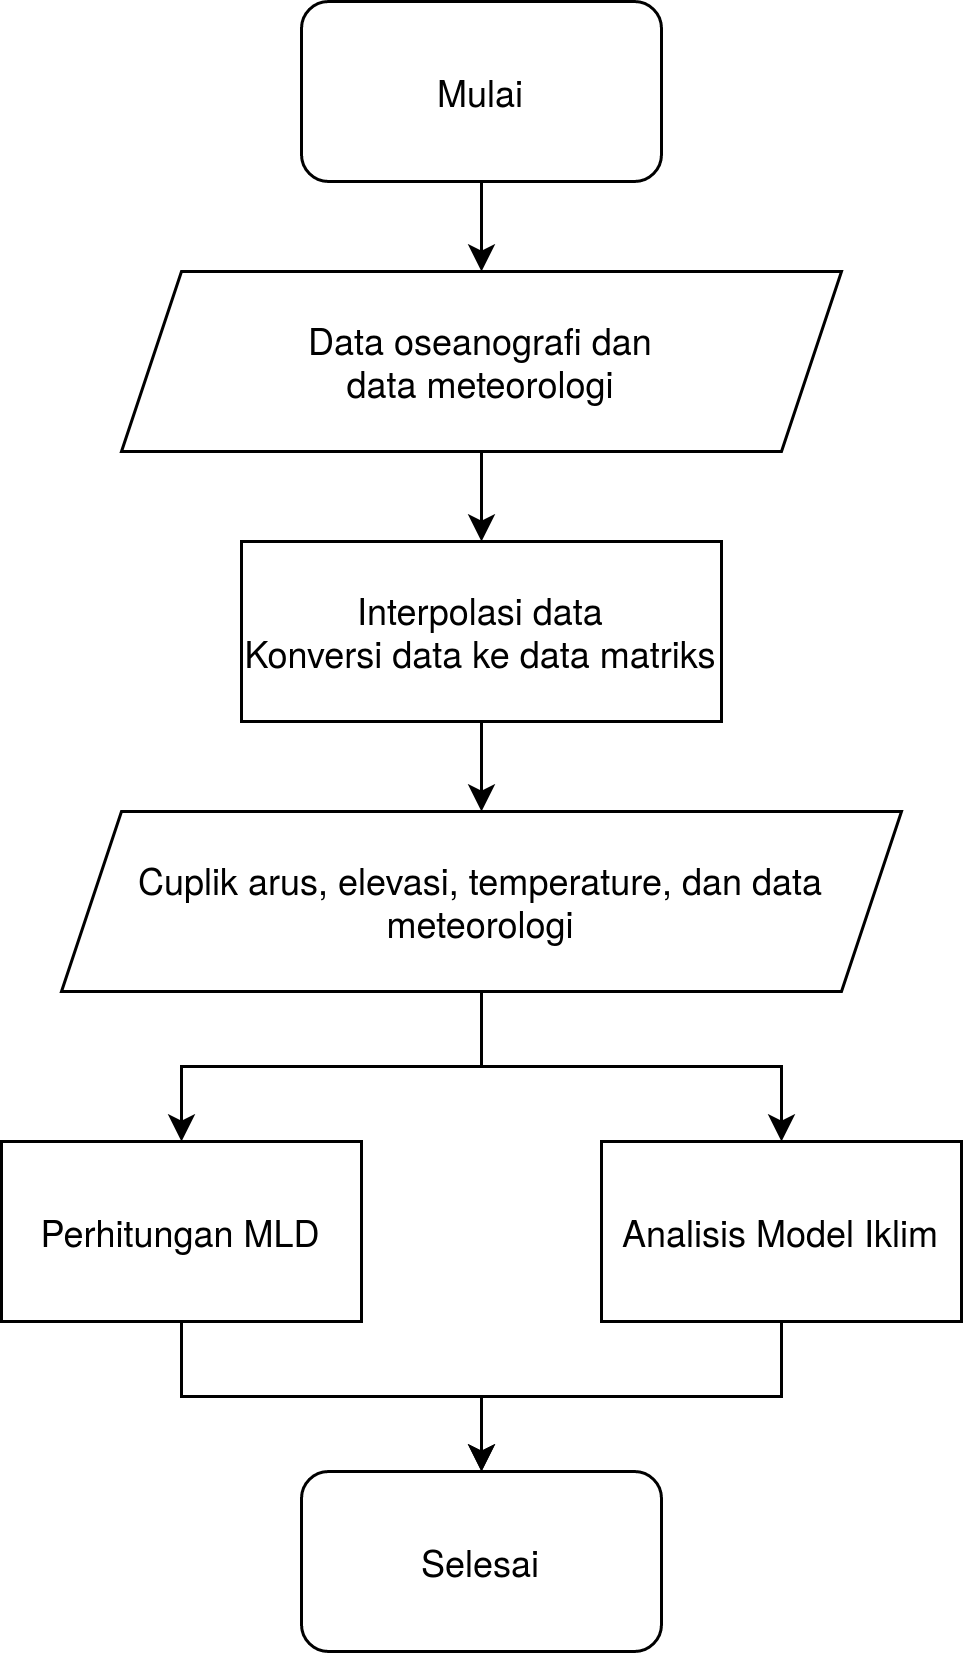
\includegraphics[width=9cm]{flowchart.png}
		\caption{Diagram alir penelitian}
		\label{fig:flowchart}
	\end{figure}
\end{frame}
\ThankYouFrame

\end{document}